\documentclass[12pt]{article}
\newif\ifanswer\answertrue%\answerfalse% comment out to show/hide answers
\usepackage{../preamble3}% preamble always after \newif\ifanswer
%\pagenumbering{gobble}
\title{Art Of Problem Solving - AMC 10 \\ Week 12}
\author{Patrick \& James Toche}
\date{August 28, 2021}

\begin{document}
\maketitle
\begin{minipage}{\textwidth}
\begin{abstract}\setlength{\parindent}{0pt}%
Notes on the AMC-10 Course by Art Of Problem Solving (AOPS).
Copyright restrictions may apply. Written for personal use. 
Please report typos and errors over at \url{https://github.com/ptoche/Math/tree/master/aops}. 
\end{abstract}
\end{minipage}

\thispagestyle{empty}
\clearpage


%%%%%%%%%%%%%%%%%%%%%%%%%%%%%%%%%%%%%%%%%%%%%%%%%%%%%%%%%%%%%%%%%%%%%%%%
\subsection*{1.}

\nopagebreak

A parabola with equation $y=x^2+bx+c$ passes through the points $(2,3)$ and $(4,3)$. What is $c$?

\nopagebreak

\fbox{(A) $2$ \quad (B) $5$ \quad (C) $7$ \quad (D) $10$ \quad (E) $11$}

\begin{answer}
Substituting the points $(2,3)$ and $(4,3)$ into $y = x^2 + bx + c$, we obtain the system of equations
\begin{align*} 
 4 + 2b + c & = 3 \\ 
16 + 4b + c & = 3 
\end{align*}
These equations simplify to
\begin{align*} 
2b + c & = -1 \\ 
4b + c & = -13 
\end{align*}
Multiplying the first equation by $2$, we get $4b + 2c = -2$. Subtracting the equation $4b + c = -13$, we get $c=11$. 
\begin{empheq}[box={\mathbox[colback=white]}]{equation*}
    c = 11
\end{empheq} 
\end{answer}
%%%%%%%%%%%%%%%%%%%%%%%%%%%%%%%%%%%%%%%%%%%%%%%%%%%%%%%%%%%%%%%%%%%%%%%%

\iftoggle{showAnswers}{\newpage}

%%%%%%%%%%%%%%%%%%%%%%%%%%%%%%%%%%%%%%%%%%%%%%%%%%%%%%%%%%%%%%%%%%%%%%%%
\subsection*{2.}

\nopagebreak

If $a$, $b > 0$ and the triangle in the first quadrant bounded by the coordinate axes and the graph of $ax+by=6$ has area 6, then $ab=$

\nopagebreak

\fbox{(A) $3$ \quad (B) $6$ \quad (C) $12$ \quad (D) $108$ \quad (E) $432$}

\begin{answer}
Setting $y=0$ we have that the $x-$intercept of the line is $x=6/a$. Similarly setting $x=0$ we find the $y-$intercept to be $y=6/b$. Then 
\begin{align*} 
\frac{1}{2} \cdot \frac{6}{a} \cdot \frac{6}{b} = \frac{18}{ab} = 6
\implies
ab = 3
\end{align*}
\begin{empheq}[box={\mathbox[colback=white]}]{equation*}
    ab = 3
\end{empheq} 
\end{answer}
%%%%%%%%%%%%%%%%%%%%%%%%%%%%%%%%%%%%%%%%%%%%%%%%%%%%%%%%%%%%%%%%%%%%%%%%

\iftoggle{showAnswers}{\newpage}

%%%%%%%%%%%%%%%%%%%%%%%%%%%%%%%%%%%%%%%%%%%%%%%%%%%%%%%%%%%%%%%%%%%%%%%%
\subsection*{3.}

\nopagebreak

The lines $x=\dfrac{1}{4}y+a$ and $y=\dfrac{1}{4}x+b$ intersect at the point $(1,2)$. What is $a+b$?

\nopagebreak

\fbox{(A) $0$ \quad (B) $\dfrac{3}{4}$ \quad (C) $1$ \quad (D) $2$ \quad (E) $\dfrac{9}{4}$}

\begin{answer}
\begin{align*}
\begin{cases}
x = \dfrac{1}{4} y + a \\[3ex] 
y = \dfrac{1}{4} x + b 
\end{cases}
\end{align*}
Add both equations and rearrange:
\begin{align*}
x+y = \frac{1}{4}(x+y) + a+b
\implies
\frac{3}{4}(x+y) = a+b 
\end{align*}
Substitute the intersection point $(1,2)$:
\begin{align*}
a+b = \frac{3}{4} \cdot (1+2)
    = \frac{9}{4}
\end{align*}
\begin{empheq}[box={\mathbox[colback=white]}]{equation*}
    a+b = \frac{9}{4}
\end{empheq} 
\end{answer}
%%%%%%%%%%%%%%%%%%%%%%%%%%%%%%%%%%%%%%%%%%%%%%%%%%%%%%%%%%%%%%%%%%%%%%%%

\iftoggle{showAnswers}{\newpage}

%%%%%%%%%%%%%%%%%%%%%%%%%%%%%%%%%%%%%%%%%%%%%%%%%%%%%%%%%%%%%%%%%%%%%%%%
\subsection*{4.}

\nopagebreak

Triangle $OAB$ has $O=(0,0)$, $B=(5,0)$, and $A$ in the first quadrant. In addition, $\angle ABO=90^\circ$ and $\angle AOB=30^\circ$. Suppose that $\overline{OA}$ is rotated $90^\circ$ counterclockwise about $O$. What are the coordinates of the image of $A$?

\nopagebreak

\fbox{(A) $\left(-\dfrac{10}{3}\sqrt{3},5\right)$ \quad (B) $\left(-\dfrac{5}{3}\sqrt{3},5\right)$ \quad (C) $\left(\sqrt{3},5\right)$ \quad (D) $\left(\dfrac{5}{3}\sqrt{3},5\right)$ \quad (E) $\left(\dfrac{10}{3}\sqrt{3},5\right)$}

\begin{answer}
\begin{center}
  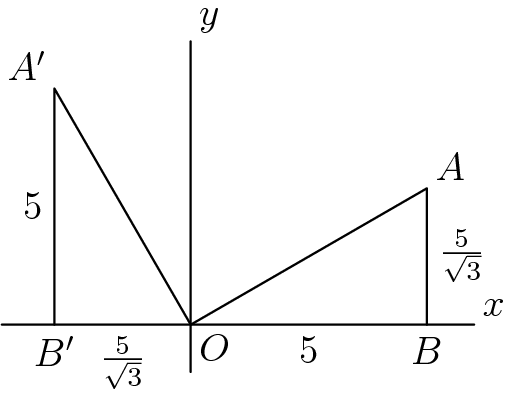
\includegraphics[height=5cm,page=1]{2021-08-28-figure-04}
\end{center}
Triangle $\triangle ABO$ is a special $30$-$60$-$90$ triangle, with $\angle ABO=90^\circ$, and $\angle AOB=30^\circ$. Since $B$ has coordinates $(5,0)$, we have $OB=5$. The triangle's proportions imply
\begin{align*}
\frac{5}{\sqrt{3}} = \frac{AB}{1}
\implies 
AB = \frac{5\sqrt{3}}{3}
\end{align*}
$A$ has coordinates $\left(5,\dfrac{5\sqrt{3}}{3}\right)$.

Rotating triangle $\triangle ABO$ by $90^\circ$ counterclockwise around $O$ takes $A$ to:
\begin{empheq}[box={\mathbox[colback=white]}]{equation*}
    \left(-\frac{5\sqrt{3}}{3},5\right)
\end{empheq} 
\end{answer}
%%%%%%%%%%%%%%%%%%%%%%%%%%%%%%%%%%%%%%%%%%%%%%%%%%%%%%%%%%%%%%%%%%%%%%%%

\iftoggle{showAnswers}{\newpage}

%%%%%%%%%%%%%%%%%%%%%%%%%%%%%%%%%%%%%%%%%%%%%%%%%%%%%%%%%%%%%%%%%%%%%%%%
\subsection*{5.}

\nopagebreak

The diagram shows 28 lattice points, each one unit from its nearest neighbors. Segment $AB$ meets segment $CD$ at $E$. Find the length of segment $AE$.

\nopagebreak

\begin{center}
  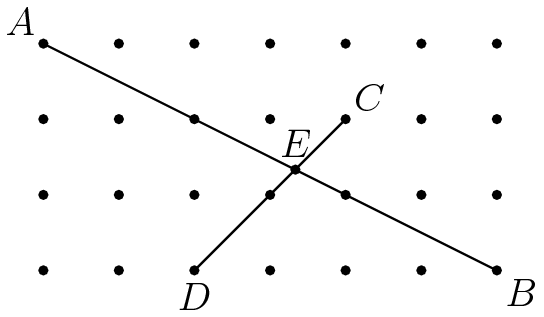
\includegraphics[height=5cm,page=1]{2021-08-28-figure-05}
\end{center}

\fbox{(A) $4\sqrt{5}/3$  \quad (B) $5\sqrt{5}/3$ \quad (C) $12\sqrt{5}/7$ \quad (D) $2\sqrt{5}$ \quad (E) $5\sqrt{65}/9$}

\begin{answer}
\subsubsection*{Solution 1}
Let $CD$ and the line through $A$ parallel to $BD$ intersect at $F$.
\begin{center}
  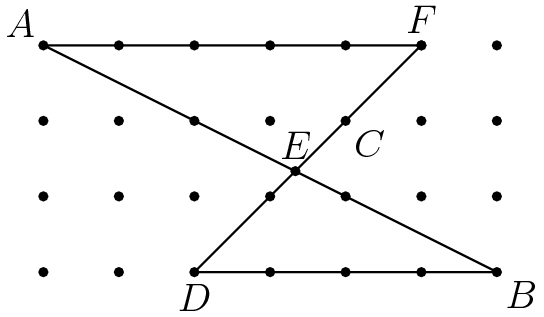
\includegraphics[height=4cm,page=1]{2021-08-28-figure-05b}
\end{center}
Then triangles $AEF$ and $BED$ are similar, so
\begin{align*}
\frac{AE}{BE} = \frac{AF}{BD}
\implies 
\frac{AE}{AE + BE} = \frac{AF}{AF + BD} \\
\implies 
AE + BE = AB = \sqrt{6^2 + 3^2} = \sqrt{45} = 3 \sqrt{5} \\
\implies 
AE = AB \cdot \frac{AF}{AF + BD} = 3 \sqrt{5} \cdot \frac{5}{5 + 4} 
= \frac{5 \sqrt{5}}{3}
\end{align*}
\begin{empheq}[box={\mathbox[colback=white]}]{equation*}
    AE = \frac{5\sqrt{5}}{3}
\end{empheq} 
\end{answer}

\begin{answer}
\newpage 
\subsubsection*{Solution 2}
\begin{center}
  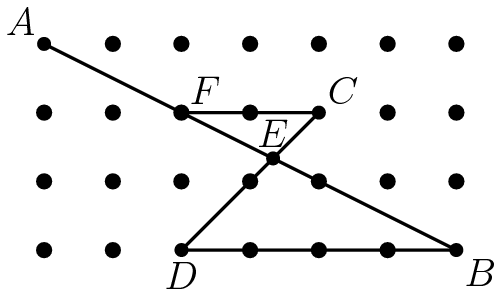
\includegraphics[height=4cm,page=1]{2021-08-28-figure-05c}
\end{center}
Draw segment $BD$ and parallel line $CF$. Since triangles $\triangle FCE$ and $\triangle BDE$ are similar,
\begin{align*}
\frac{FE}{EB} 
  = \frac{FC}{DB} 
  = \frac{2}{4} 
  = \frac{1}{2}
\implies
\frac{EB+FE}{FE} 
  = 2+1 
  \implies 
FE = \frac{1}{3}FB
\end{align*}
By construction, $FD = 2$. Applying the Pythagorean Theorem to $\triangle BDF$,
\begin{align*}
FB = \sqrt{2^{2} + 4^{2}} 
   = 2\sqrt{5}
\implies 
FE = \frac{1}{3}FB 
   = \frac{2\sqrt{5}}{3}
\end{align*}
Applying the Pythagorean Theorem,
\begin{align*}
AF = \sqrt{1^{2}+2^{2}} 
   = \sqrt{5}
\end{align*}
Adding it up,
\begin{align*}
AE = AF + FE 
   = \sqrt{5} + \frac{2\sqrt{5}}{3} 
   = \frac{5\sqrt{5}}{3}
\end{align*}
\begin{empheq}[box={\mathbox[colback=white]}]{equation*}
    AE = \frac{5\sqrt{5}}{3}
\end{empheq} 
\end{answer}
%%%%%%%%%%%%%%%%%%%%%%%%%%%%%%%%%%%%%%%%%%%%%%%%%%%%%%%%%%%%%%%%%%%%%%%%

%\iftoggle{showAnswers}{\newpage}
\newpage% tweaked

%%%%%%%%%%%%%%%%%%%%%%%%%%%%%%%%%%%%%%%%%%%%%%%%%%%%%%%%%%%%%%%%%%%%%%%%
\subsection*{6.}

\nopagebreak

Five unit squares are arranged in the coordinate plane as shown, with the lower left corner at the origin. The slanted line, extending from $(a,0)$ to $(3,3)$, divides the entire region into two regions of equal area. What is $a$?

\nopagebreak

\begin{center}
  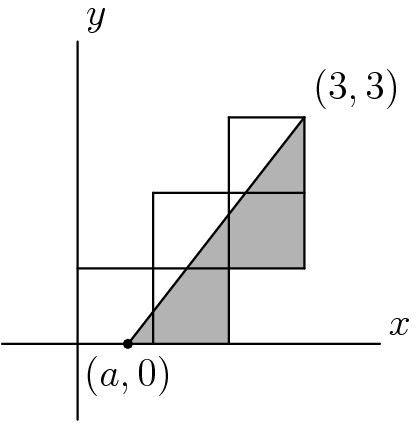
\includegraphics[height=5cm,page=1]{2021-08-28-figure-06}
\end{center}

\fbox{(A) $\dfrac{1}{2}$ \quad (B) $\dfrac{3}{5}$ \quad (C) $\dfrac{2}{3}$ \quad (D) $\dfrac{3}{4}$ \quad (E) $\dfrac{4}{5}$}

\begin{answer}
If one unit square is added to the bottom-right corner, the shaded area has the shape of a triangle with base length $3-a$, height $3$, and therefore area $(9-3a)/2$. 

If three unit squares are added to the top-left corner, the unshaded area has the shape of a trapezoid with area $(9+3a)/2$. 

The shaded and unshaded areas are equal:
\begin{align*}
\frac{9-3a}{2} -1 = \frac{9+3a}{2} -3
\implies 
a = \frac{2}{3}
\end{align*}
\begin{empheq}[box={\mathbox[colback=white]}]{equation*}
    a = \frac{2}{3}
\end{empheq} 
\end{answer}
%%%%%%%%%%%%%%%%%%%%%%%%%%%%%%%%%%%%%%%%%%%%%%%%%%%%%%%%%%%%%%%%%%%%%%%%

\iftoggle{showAnswers}{\newpage}

%%%%%%%%%%%%%%%%%%%%%%%%%%%%%%%%%%%%%%%%%%%%%%%%%%%%%%%%%%%%%%%%%%%%%%%%
\subsection*{7.}

\nopagebreak

In rectangle $ABCD$, we have $A = (6,-22)$, $B = (2006,178)$, and $D = (8,y)$, for some integer $y$. What is the area of rectangle $ABCD$?

\nopagebreak

\fbox{(A) $4000$ \quad (B) $4040$ \quad (C) $4400$ \quad (D) $40,000$ \quad (E) $40,400$}

\begin{answer}
Let the slope of $AB$ be $m_1$ and the slope of $AD$ be $m_2$.
\begin{align*}
m_1 & = \frac{178-(-22)}{2006-6} = \frac{1}{10} \\[1ex]
m_2 & = \frac{y-(-22)}{8-6} = \frac{y+22}{2}
\end{align*}
Since $AB$ and $AD$ form a right angle:
\begin{align*}
m_2 & = -\frac{1}{m_1} \\[1ex]
m_2 & = -10 \\[1ex]
\frac{y+22}{2} & = -10 \\[1ex]
y & = -42
\end{align*}
Using the distance formula:
\begin{align*}
AB & = \sqrt{(2006-6)^2 + (178-(-22))^2} \\[1ex]
   & = \sqrt{(2000)^2 + (200)^2} \\[1ex]
   & = 200\sqrt{101} \\[1ex]
AD & = \sqrt{(8-6)^2 + (-42-(-22))^2} \\[1ex]
   & = \sqrt{(2)^2 + (-20)^2} \\[1ex]
   & = 2\sqrt{101}
\end{align*}
Therefore the area of rectangle $ABCD$ is 
\begin{align*}
200\sqrt{101}\cdot2\sqrt{101} = 40,400
\end{align*}
\begin{empheq}[box={\mathbox[colback=white]}]{equation*}
    \text{area}~ = 40,400
\end{empheq} 
\end{answer}
%%%%%%%%%%%%%%%%%%%%%%%%%%%%%%%%%%%%%%%%%%%%%%%%%%%%%%%%%%%%%%%%%%%%%%%%

\iftoggle{showAnswers}{\newpage}

%%%%%%%%%%%%%%%%%%%%%%%%%%%%%%%%%%%%%%%%%%%%%%%%%%%%%%%%%%%%%%%%%%%%%%%%
\subsection*{8.}

\nopagebreak

If $(a,b)$ and $(c,d)$ are two points on the line whose equation is $y = mx + k$, then the distance between $(a,b)$ and $(c,d)$, in terms of $a$, $c$, and $m$, is

\nopagebreak

\fbox{(A) $|a-c|\sqrt{1+m^2}$ \quad (B)  $|a+c|\sqrt{1+m^2}$  \quad (C) $\dfrac{|a-c|}{\sqrt{1+m^2}}$  \quad (D) $|a-c|(1+m^2)$  \quad (E) $|a-c||m|$ }

\begin{answer}
Notice that, since $(a, b)$ is on $y=mx+k$, we have $b=am+k$. Similarly, $d=cm+k$. Using the distance formula, the distance between the points $(a, b)$ and $(c, d)$ is
\begin{align*}
\sqrt{(a-c)^2+(b-d)^2}
& = \sqrt{(a-c)^2+[(am+k)-(cm+k)]^2} \\
& = \sqrt{(a-c)^2+m^2(a-c)^2} \\
& = |a-c|\sqrt{1+m^2}
\end{align*}
\begin{empheq}[box={\mathbox[colback=white]}]{equation*}
    |a-c|\sqrt{1+m^2}
\end{empheq} 
\end{answer}
%%%%%%%%%%%%%%%%%%%%%%%%%%%%%%%%%%%%%%%%%%%%%%%%%%%%%%%%%%%%%%%%%%%%%%%%

\iftoggle{showAnswers}{\newpage}

%%%%%%%%%%%%%%%%%%%%%%%%%%%%%%%%%%%%%%%%%%%%%%%%%%%%%%%%%%%%%%%%%%%%%%%%
\subsection*{9.}

\nopagebreak

A lattice point is a point in the plane with integer coordinates. How many lattice points are on the line segment whose endpoints are $(3,17)$ and $(48,281)$? (Include both endpoints of the segment in your count.)

\nopagebreak

\fbox{(A) $2$ \quad (B) $4$ \quad (C) $6$ \quad (D) $16$ \quad (E) $46$}

\begin{answer}
The difference in the $y$-coordinates is $281 - 17 = 264$, and the difference in the $x$-coordinates is $48 - 3 = 45$. The gcd of 264 and 45 is 3, so the line segment joining $(3,17)$ and $(48,281)$ has slope $\dfrac{88}{15}$. The points on the line have coordinates
\begin{align*}
\left(3+t,~17+\frac{88}{15}t\right)
\end{align*}
If $t$ is an integer, the $y$-coordinate of this point is an integer if and only if $t$ is a multiple of 15. The points where $t$ is a multiple of 15 on the segment $3\leq x\leq 48$ are $3$, $3+15$, $3+30$, and $3+45$. There are 4 lattice points on this line. 
\begin{empheq}[box={\mathbox[colback=white]}]{equation*}
    4 ~\text{lattice points}
\end{empheq} 
\end{answer}
%%%%%%%%%%%%%%%%%%%%%%%%%%%%%%%%%%%%%%%%%%%%%%%%%%%%%%%%%%%%%%%%%%%%%%%%

\iftoggle{showAnswers}{\newpage}

%%%%%%%%%%%%%%%%%%%%%%%%%%%%%%%%%%%%%%%%%%%%%%%%%%%%%%%%%%%%%%%%%%%%%%%%
\subsection*{10.}

\nopagebreak

The number of distinct points in the $xy$-plane common to the graphs of $(x + y - 5)(2x - 3y + 5) = 0$ and $(x -y + 1)(3x + 2y - 12) = 0$ is

\nopagebreak

\fbox{(A) $0$ \quad (B) $1$ \quad (C) $2$ \quad (D) $3$ \quad (E) $4$}

\begin{answer}
\begin{center}
  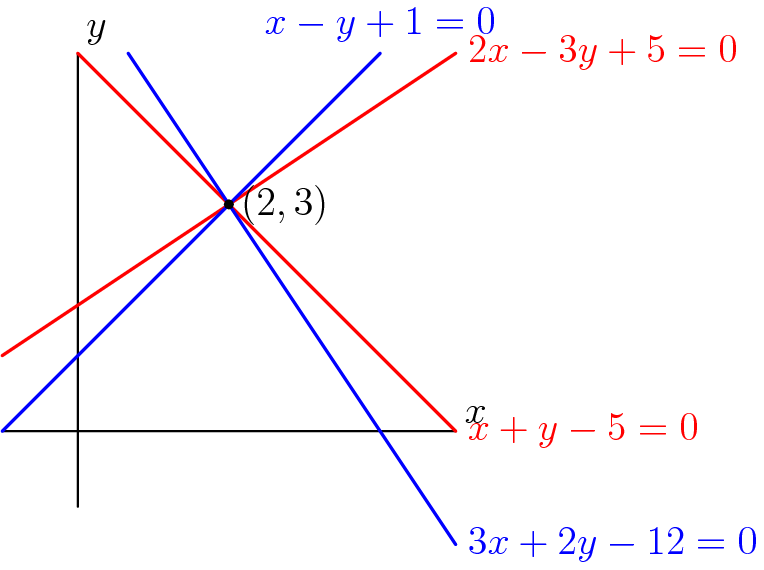
\includegraphics[height=7cm,page=1]{2021-08-28-figure-10}
\end{center}
The graph $(x + y - 5)(2x - 3y + 5) = 0$ is the combined graphs of $x + y - 5=0$ and $2x - 3y + 5 = 0$. Likewise, the graph $(x -y + 1)(3x + 2y - 12) = 0$ is the combined graphs of $x-y+1=0$ and $3x+2y-12=0$. All these lines intersect at one point, $(2,3)$. Therefore, the answer is $1$. 
\begin{empheq}[box={\mathbox[colback=white]}]{equation*}
    1 ~\text{distinct point}
\end{empheq} 
\end{answer}
%%%%%%%%%%%%%%%%%%%%%%%%%%%%%%%%%%%%%%%%%%%%%%%%%%%%%%%%%%%%%%%%%%%%%%%%


\end{document}
